\documentclass{astroedu-lab}

\begin{document}

\pagestyle{plain}

\begin{problem}{\huge Лабораторная работа 3.2.3\\\\Резонанс токов в параллельном\\\\контуре\\\\Выполнил Жданов Елисей Б01-205}

\section{Цель работы:}

1) Исследование резонанса токов в параллельном колебательном
контуре с изменяемой индуктивностью, получение амплитудно-частотных и фазово-частотных характеристик контура

2) Определение основных параметров контура


\section{Оборудование:}

1) Лабораторный автотрансформатор (ЛАТР)

2) Разделительный понижающий трансформатор

3) Конденсатор

4) Катушка с переменной индуктивностью(дроссель)

5) Три амперметра

6) Вольтметр

7) Реостат

8) Электронный осциллограф

9) Мультиметр (LCR)

10) Мост переменного тока

\newpage

\section{Теоретическая справка}

В работе изучается параллельный контур, одна из ветвей которого содержит индуктивность L, другая — ёмкость C. Через rL обозначено активное сопротивление катушки, которое включает в себя как чисто омическое сопротивление витков катушки, так и сопротивление, связанное с потерями энергии при перемагничивании сердечника катушки. Активным сопротивлением емкостной ветви контура можно пренебречь.

\section{Экспериментальная установка}

\begin{figure}[!h]
	\centering
	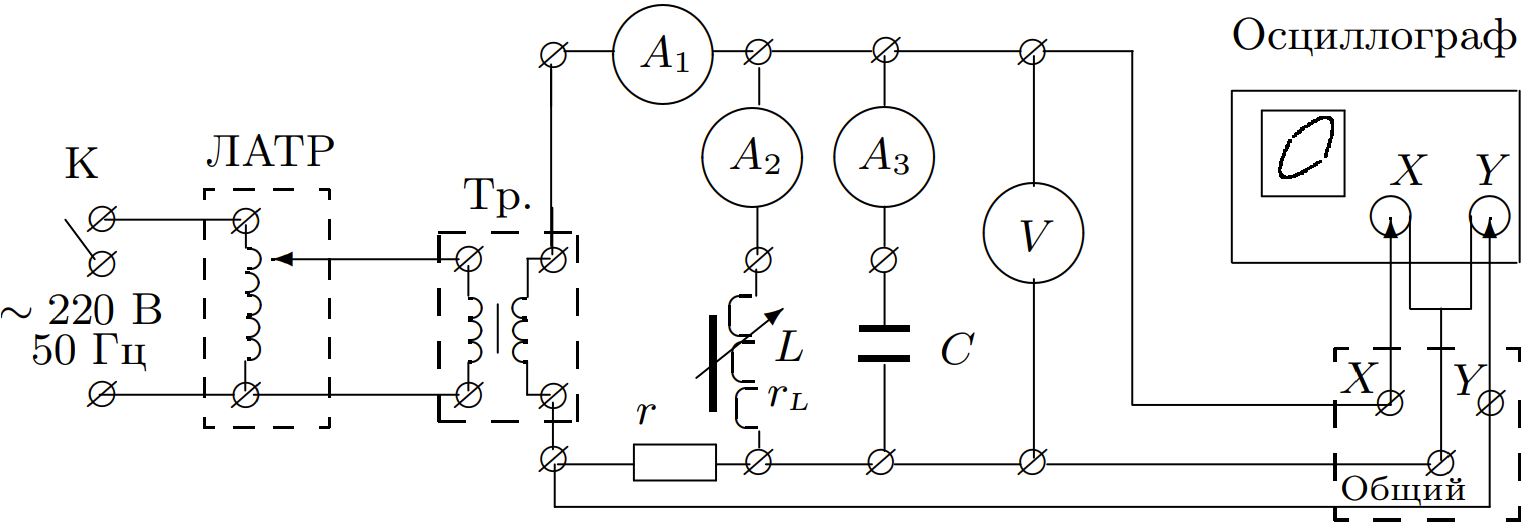
\includegraphics[width=0.9\textwidth]{установка.png}
	\label{fig:boiler}
\end{figure}

Напряжение от сети (220 В, 50 Гц) с помощью ЛАТРа через понижающий трансформатор Тр подаётся на параллельный
контур, содержащий конденсатор (C = 120 мкФ) и катушку, индуктивность которой зависит от глубины погружения сердечника. Полный ток в цепи измеряется с помощью амперметра A1; для измерения токов в L- и C-ветвях используются два одинаковых амперметра A2 и A3; напряжение на контуре контролируется вольтметром V. Последовательно с контуром включён резистор-реостат (r = 100 Ом).


Для наблюдения за сдвигом фаз между полным током и напряжением
на контуре используется осциллограф. Сигнал, пропорциональный току, снимается с резистора r и подаётся на вход Y осциллографа. На вход X подаётся напряжение непосредственно с контура. При наличии сдвига фаз между этими напряжениями на экране виден эллипс, а при нулевом сдвиге фаз эллипс вырождается в прямую.

\newpage

\section{Измерения, Обработка}

\subsection{Выполнение}

1) Подготовим установку к эксперименту: включим все измерительные приборы и питание и опустим сердечник индуктивности до конца.

2) При напряжении контура U = 5 В во всем диапазоне индуктивности, ток в контуре не превышает 0.5 А. Будем фиксировать это напряжение при каждом замере.

Результаты измерений приведены в таблице ниже.

\begin{center}
	\Large $U = 5 \text{ В}$
\end{center}

\begin{center}
\begin{tabular}{|c|c|c|c|}
\hline 
h, см & $I(A_1)$, мА & $I_L(A_2)$, мА & $I_C(A_3)$, мА \\
\hline
13.1 & 380 & 605 & 220 \\
12   & 275 & 490 & 210 \\
11   & 215 & 460 & 210 \\
10   & 140 & 350 & 210 \\
9	 & 95  & 320 & 220 \\
8	 & 25  & 270 & 220 \\
7	 & 0   & 230 & 220 \\
6	 & 0   & 200 & 220 \\
5	 & 25  & 100 & 200 \\
4	 & 50  & 90  & 210 \\
3	 & 90  & 60  & 205 \\
2	 & 110 & 90  & 205 \\
1	 & 130 & 20  & 205 \\
0	 & 155 & 0   & 205 \\

\hline
\end{tabular}
\end{center}

Также приведем сводную таблицу характеристик схемы.

\begin{center}
\begin{tabular}{|c|c|}
\hline 
C &		120 мкФ	\\
r & 	100	Ом	\\
$\nu$ & 50  Гц	\\
\hline
\end{tabular}
\end{center}

Резонанс наблюдается при параметрах(U = 10 В):

\begin{center}
\begin{tabular}{|c|c|}
\hline 
U & 10		 В  \\
h & 71		 мм \\
I & 2.5		 мА \\
$I_L$ & 44.5 мА \\
$I_C$ & 44   мА \\
\hline
\end{tabular}
\end{center}

3-4) Для точного измерения резонанса перейдем на повышенное напряжение, поскольку при U = 5 В улучшение точности более невозможно. Добъемся выпрямления резонансной прямой на осциллографе в центральной точке и поднимем напряжение до 20 В. Полученные значения приведены ниже.

\begin{center}
\begin{tabular}{|c|c|}
\hline 
U & 20		В  \\
h & 70		мм \\
I & 80		мА \\
$I_L$ & 780	мА \\
$I_C$ & 800	мА \\
\hline
\end{tabular}
\end{center}

5-8) Отключим питание и подключим мультиметр к катушке.

9) Замеры мультиметром сведены в таблицу

\begin{center}
\begin{tabular}{|c|c|c|}
\hline 
$\nu$ 		& 1 кГц & 50 Гц \\
\hline 
$L_s$, мГн	& 70.77 & 76.93	\\
$R_s$, Ом	& 34.2	& 1.683	\\
\hline
\end{tabular}
\end{center}

10) Добротность контура

\begin{equation}
	Q = \frac{I_\text{С, рез}}{I_\text{рез}} = 10 \pm 1
\end{equation}

Резонансное сопротивление контура

\begin{equation}
	R_\text{рез} = \frac{U_0}{I_\text{рез}} = 250 \pm 30 \text{ Ом}
\end{equation}

Формула для $R_\text{рез}$ из теории

\begin{equation}
	R_\text{т. рез} = \frac{L / C}{\sqrt{r_L^2 + \left( \frac{1}{\omega C} - \omega L \right)^2}} = 220 \text{ Ом}
\end{equation}

Как видно, результаты весьма близкие в рамках погрешности. Более подробно о различии указано в выводе.

\newpage

\subsection{Обработка}

1) График

\begin{figure}[!h]
	\centering
	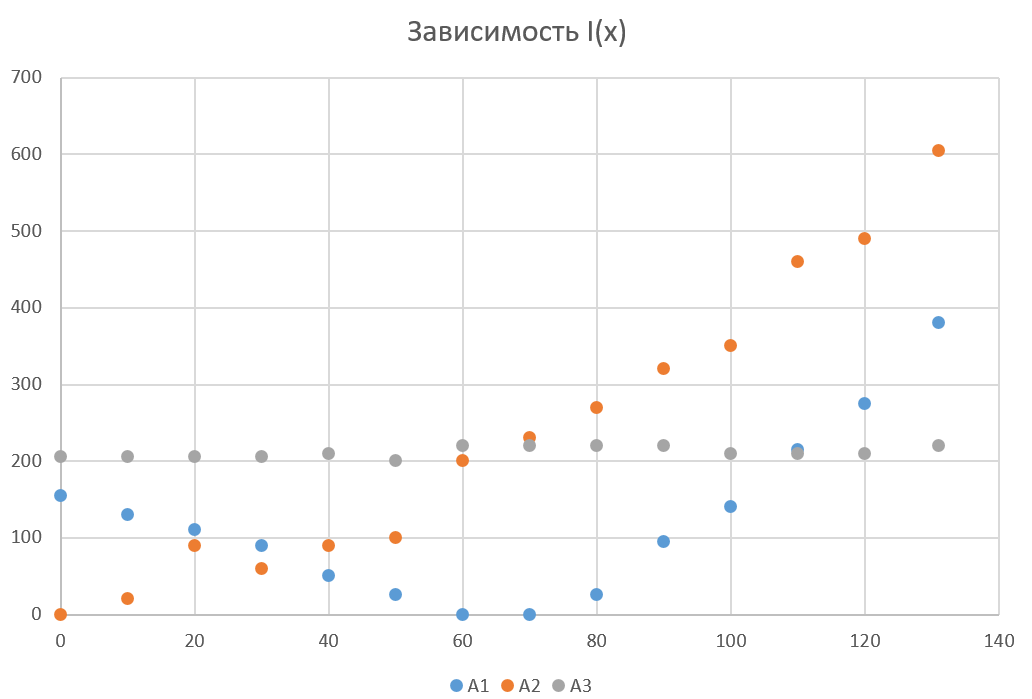
\includegraphics[width=0.9\textwidth]{Ix.png}
	\label{fig:boiler}
\end{figure}

2-3) Рассчитаем по формулам из источника.

\begin{equation}
	L_\text{рез} = \frac{1}{\omega^2 C} = 84.4 \text{ мГн}
\end{equation}

\begin{equation}
	r_\text{L} = \frac{1}{Q \omega С} = 2.7 \pm 0.3 \text{ Ом}
\end{equation}

4) И также резонансный ток

\begin{equation}
	L_\text{рез} = \frac{U}{I_\text{L рез} \omega} = 80 \pm 10 \text{ мГн}
\end{equation}

\newpage

5) Диаграмма

\begin{figure}[!h]
	\centering
	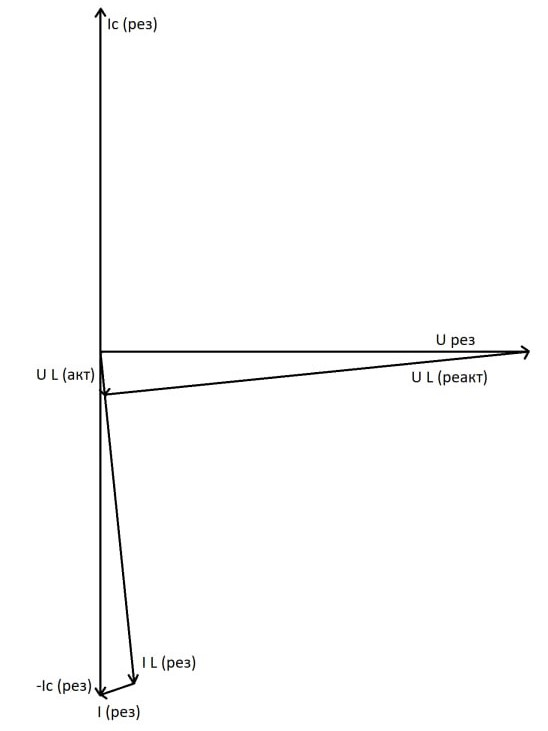
\includegraphics[width=0.5\textwidth]{vector.jpg}
	\label{fig:boiler}
\end{figure}

Итого $U_\text{L акт} = 2.1 \text{ В}$, а $U_\text{L реакт} = 20 \text{ В}$. Наконец $r_L = \frac{U_\text{L акт}}{I_\text{L рез}} = 2.5 \text{ Ом}$, а $L_{\text{рез}} = 0.08 \text{ мГн}$.

Итоговая таблица

\begin{center}
\begin{tabular}{|c|c|c|c|c|}
\hline 
& Мультиметр & f($\omega$, C, Q) & f(U, I) & Диаграмма \\
\hline 
$r_L$, Ом			& 1.683 & 2.7 $\pm$ 0.3	& - & 2.5\\
\hline
$L_\text{рез}$, мГн	& 76.93	& 84.4 & 80 $\pm$ 10 & 80\\
\hline
\end{tabular}
\end{center}

\section{Вывод}

Реактивное сопротивление колебательного контура в резонансе довольно близко с теоретическому расчету. Значения $L_\text{рез}$ также оказались довольно близко совпадающими. Напротив, значения $r_L$ разнятся довольно сильно. В основном, все возможные неточности вызваны дифференциальностью метода оценки значений: поскольку резонансная точка довольно трудно уловима, характеристики контура вблизи неё меняются в довольно широких пределах. Также следует заметить, что осциллограмма не вырождалась в математическую прямую, а имела форму тонкой восьмерки с заметными буграми. Это означает не только то, что в цепи могут быть неучтенные сопротивления(например, питания), но и неидеальность компонент, а именно зависимости емкости или индуктивности от тока в контуре. Тем не менее, значения измерений сходятся по порядку, что подтверждает разумность теоретических предположений.


\end{problem}
\end{document}